\subsection{ Makrozyklus Schritt 1: Zustandssimulation und Datengenerierung}

Die Generierung der Schaltungszustände, die als Input für den Lernprozess dienen, erfolgt mittels einer Zufallsfunktion. In der realen Welt erfolgen Zustandsübergänge in einer physischen Schaltung in langen Zeitintervallen, was eine direkte Simulation unpraktisch macht. Deshalb greifen wir auf eine alternative Methode zurück:

\begin{itemize}
    \item Initial wird über eine Gleichverteilung ein Degenerationszustand der Schaltung simuliert. Die zufällige Auswahl dieser Zustände geschieht innerhalb festgelegter Grenzen, um eine Vielfalt an möglichen Zuständen zu gewährleisten.
	\item Der simulierte Zustand wird durch einen Satz von Kapazitäts- und Induktivitätswerten dargestellt. Diese Werte werden durch den "Würfel" im System visualisiert \ref{fig:state_generation}, wobei die Pfeile vom Würfel zu den Zustandsvariablen C und L diesen Prozess der zufälligen Zustandsgenerierung abbilden.
\end{itemize}

In diesem Projekt werden exemplarische Einstellungen für die Zustandsgenerierung verwendet, die eine Annäherung an realitätsnahe Bedingungen darstellen. Bei einer Überführung in praktische Anwendungen würden diese Einstellungen so angepasst, dass sie mit den in der Realität verifizierten Werten übereinstimmen. Die aktuellen Grenzwerte für die Zustandsgenerierung sind wie folgt definiert:

\begin{itemize}
    \item Untergrenze: \( \text{Induktivität} = 5.0 \times 10^{-4} \), \( \text{Kapazität} = 1.0 \times 10^{-6} \)
    \item Obergrenze: \( \text{Induktivität} = 5.0 \times 10^{-2} \), \( \text{Kapazität} = 1.0 \times 10^{-4} \)
\end{itemize}

\begin{figure}[htbp]
\centering
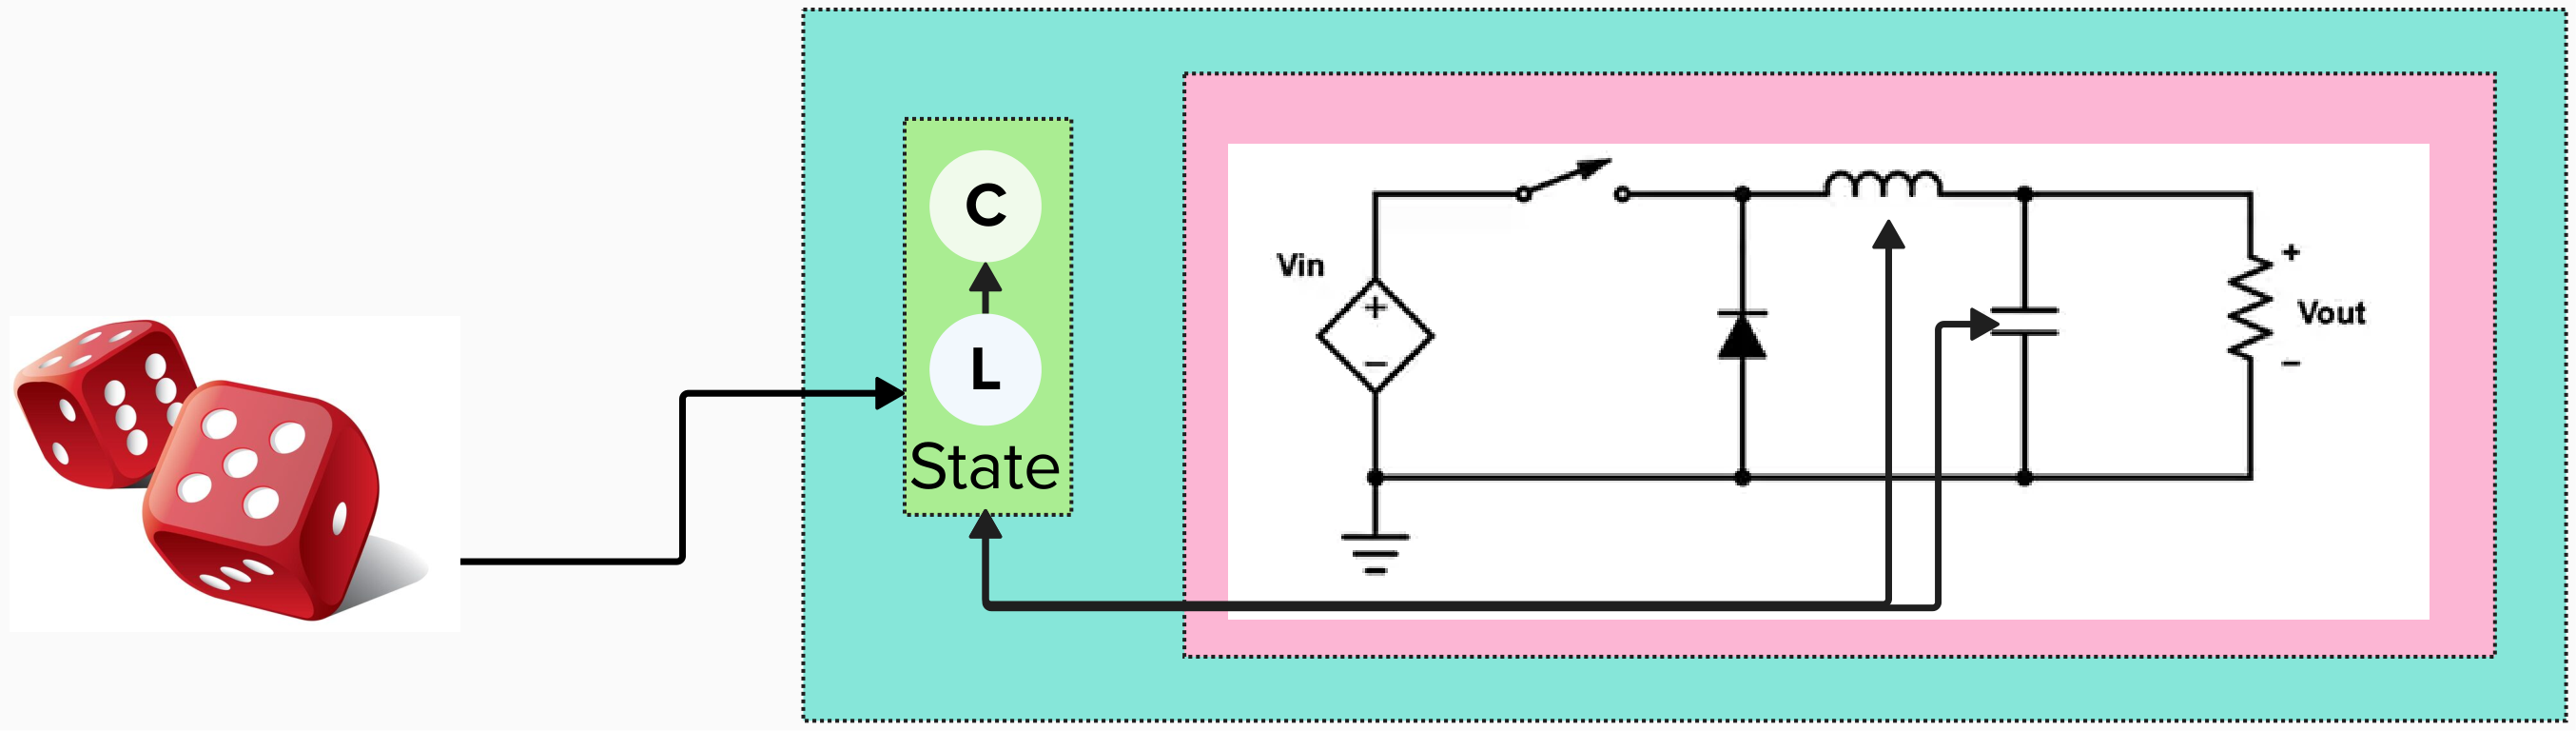
\includegraphics[width=0.7\textwidth]{3Experiment/2Experiment/1Random_Set_State.png}
\caption{Visualisierung der Zustandsgenerierung mit dem Würfel und die Setzung der Werte in der DCDC-Schaltung.}
\label{fig:state_generation}
\end{figure}
